%!TEX TS-program = xelatex
%!TEX encoding = UTF-8 Unicode
\documentclass[12pt, parindent=0]{article} % use larger type; default would be 10pt

%----------------------------------------------------------------------------------------
%   PACKAGES
%----------------------------------------------------------------------------------------
\usepackage{amsmath,amsfonts,amsthm} % Math packages
\usepackage{mathtools}
\usepackage{lipsum} % Used for inserting dummy 'Lorem ipsum' text into the template
\usepackage{datetime}
\usepackage{xfrac}
\usepackage{changepage} % for adjusting the width
\usepackage{gensymb}
\usepackage{subcaption}
\usepackage{sectsty}
\usepackage{xcolor}
\usepackage{verbatim}
\usepackage{titlesec}
\usepackage{color}
\usepackage{float} % Not have your figures fly around  - use [H]
\usepackage{booktabs} % for much better looking tables
\usepackage{array} % for better arrays (e.g matrices) in maths
\usepackage{paralist} % very flexible & customisable lists (eg. enumerate/itemize, etc.)
\usepackage{verbatim} % adds environment for commenting out blocks of text & for better verbatim
\usepackage{subfig} % make it possible to include more than one captioned figure/table in a single float
\usepackage[export]{adjustbox}
\usepackage{pdfpages} % For pdf inputs
\usepackage{import} % for subfolder inputs
\usepackage{metalogo} % for the fucking logo
\usepackage{listings}
\usepackage{mdwlist} % for tight lists
\usepackage{csquotes} % provide the \enquote command for quick quotes
%\usepackage{import} % for subfolder inputs
\usepackage{letltxmacro} % better roots
\usepackage{xspace} % for correct spacing
\usepackage{multicol} % for the multicol environment
%\usepackage{hyperref}
\usepackage{sidecap} % for sided captions
\usepackage{wrapfig}

% enable system font access
\usepackage{fontspec}
%----------------------------------------------------------------------------------------
%   FONT CONFIGURATIONS
%----------------------------------------------------------------------------------------

\setmainfont{Palatino Linotype}
\newfontfamily{\maintext}{Palatino Linotype}
\newfontfamily{\stressed}{Helvetica}
%\newfontfamily\secfont{Arial}
%\newfontfamily{\exotic}{Arial}
%\newfontfamily{\math}{Arial}
\setsansfont{Arial}

%----------------------------------------------------------------------------------------
%   DOCUMENT CONFIGURATIONS
%----------------------------------------------------------------------------------------
\definecolor{MediumBlue}{rgb}{0 ,0 ,205}
\definecolor{Blue}{rgb}{0 ,0 ,255}
\definecolor{RoyalBlue}{rgb}{65,105,225}
\definecolor{mygreen}{rgb}{0,0.6,0}
\definecolor{mygray}{rgb}{0.5,0.5,0.5}
\definecolor{mymauve}{rgb}{0.58,0,0.82}

%\titleformat*{\section}{\bfseries \color{MediumBlue}}
%\titleformat*{\subsection}{\bfseries \color{Blue}}
%\titleformat*{\subsubsection}{\bfseries \color{RoyalBlue}}
\newcommand{\en}[1] {\textenglish{#1}}

\titleformat{\paragraph}
{\normalfont\normalsize\bfseries}{\theparagraph}{1em}{}
\titlespacing*{\paragraph}
{0pt}{3.25ex plus 1ex minus .2ex}{1.5ex plus .2ex}

% New Root configuration - http://en.wikibooks.org/wiki/LaTeX/Mathematics#Roots
\LetLtxMacro{\oldsqrt}{\sqrt} % makes all sqrts closed
\renewcommand{\sqrt}[1][\ ]{%
  \def\DHLindex{#1}\mathpalette\DHLhksqrt}
\def\DHLhksqrt#1#2{%
  \setbox0=\hbox{$#1\oldsqrt[\DHLindex]{#2\,}$}\dimen0=\ht0
  \advance\dimen0-0.2\ht0
  \setbox2=\hbox{\vrule height\ht0 depth -\dimen0}%
  {\box0\lower0.71pt\box2}}

\newcommand{\norm}[1]{\lVert#1\rVert}
\newcommand{\abs}[1]{\lvert#1\rvert}
%----------------------------------------------------------------------------------------
%   GEOMETRY - GRAPHICS 
%----------------------------------------------------------------------------------------
\usepackage[a4paper, width = 150mm, top = 25mm, bottom = 25mm, bindingoffset =
5mm]{geometry} % to change the page dimensions
\usepackage{graphicx} % support the \includegraphics command and options

\graphicspath{ 
{./Drawings/CameraUploads/}
{./Drawings/MoreFigures/}
{./Drawings/Figures/}
{./Drawings/MatlabFigures/}
}

%----------------------------------------------------------------------------------------
%   LISTINGS RELATED
%----------------------------------------------------------------------------------------

\lstset{ %
  backgroundcolor=\color{white},   % choose the background color; you must add \usepackage{color} or \usepackage{xcolor}
  basicstyle=\footnotesize,        % the size of the fonts that are used for the code
  breakatwhitespace=false,         % sets if automatic breaks should only happen at whitespace
  breaklines=true,                 % sets automatic line breaking
  captionpos=b,                    % sets the caption-position to bottom
  commentstyle=\color{mygreen},    % comment style
  deletekeywords={...},            % if you want to delete keywords from the given language
  escapeinside={\%*}{*)},          % if you want to add LaTeX within your code
  extendedchars=true,              % lets you use non-ASCII characters; for 8-bits encodings only, does not work with UTF-8
  frame=none,                    % adds a frame around the code
  keepspaces=true,                 % keeps spaces in text, useful for keeping indentation of code (possibly needs columns=flexible)
  keywordstyle=\color{blue},       % keyword style
  language=Matlab,                 % the language of the code
  morekeywords={*,...},            % if you want to add more keywords to the set
  numbers=none,                    % where to put the line-numbers; possible values are (none, left, right)
  numbersep=5pt,                   % how far the line-numbers are from the code
  numberstyle=\tiny\color{mygray}, % the style that is used for the line-numbers
  rulecolor=\color{black},         % if not set, the frame-color may be changed on line-breaks within not-black text (e.g. comments (green here))
  showspaces=false,                % show spaces everywhere adding particular underscores; it overrides 'showstringspaces'
  showstringspaces=false,          % underline spaces within strings only
  showtabs=false,                  % show tabs within strings adding particular underscores
  stepnumber=2,                    % the step between two line-numbers. If it's 1, each line will be numbered
  stringstyle=\color{mymauve},     % string literal style
  tabsize=2,                       % sets default tabsize to 2 spaces
  title=\lstname                   % show the filename of files included with \lstinputlisting; also try caption instead of title
}

\newcommand{\includecode}[2][c]{\lstinputlisting[caption=#2, escapechar=, style=custom#1]{#2}}
%----------------------------------------------------------------------------------------
%   HEADER & FOOTERS
%----------------------------------------------------------------------------------------
\usepackage{fancyhdr} % This should be set AFTER setting up the page geometry
\pagestyle{fancy} % options: empty , plain , fancy
\renewcommand{\headrulewidth}{0.4pt} % customise the layout...
\lhead{\textcolor{gray}{Fligth Mechanics}\\
\textcolor{gray}{Project Work Part I}}\chead{}\rhead{}
\lfoot{}\cfoot{\thepage}\rfoot{}

%----------------------------------------------------------------------------------------
%   SECTION APPEARANCE
%----------------------------------------------------------------------------------------
% (This matches ConTeXt defaults)
\numberwithin{equation}{section} % Number equations within sections (i.e. 1.1, 1.2, 2.1, 2.2 instead of 1, 2, 3, 4)
\numberwithin{figure}{section} % Number figures within sections (i.e. 1.1, 1.2, 2.1, 2.2 instead of 1, 2, 3, 4)
\numberwithin{table}{section} % Number tables within sections (i.e. 1.1, 1.2, 2.1, 2.2 instead of 1, 2, 3, 4)

%----------------------------------------------------------------------------------------
%   TOC APPEARANCE
%----------------------------------------------------------------------------------------
\usepackage[nottoc,notlof,notlot]{tocbibind} % Put the bibliography in the ToC

%----------------------------------------------------------------------------------------
%   DOCUMENT PART
%----------------------------------------------------------------------------------------
\begin{document}
%----------------------------------------------------------------------------------------
%   TITLE SECTION
%----------------------------------------------------------------------------------------
\newcommand{\horrule}[1]{\rule{\linewidth}{#1}} % Create horizontal rule command with 1 argument of height

\begin{titlepage}

\begin{center}
\begin{figure}[htpb]
    \begin{center}
        
\includegraphics[width = 0.2\textwidth]{kth_rgb.jpg} % Just THIS!!!
    \end{center}
\end{figure}

\normalfont \normalsize 
\textsc{Royal Institute of Technology} \\  % Your university, school and/or department name(s)
\textsc{School of Engineering Sciences} \\ [25pt] % Your university, school and/or department name(s)
\horrule{0.5pt} \\[0.4cm] % Thin top horizontal rule
\huge Flight Mechanics \vspace{5mm}\\ Project Work Part \\ % The assignment title
\horrule{2pt} \\[0.5cm] % Thick bottom horizontal rule
\vspace*{10mm}

\begin{figure}[H]
    \centering
    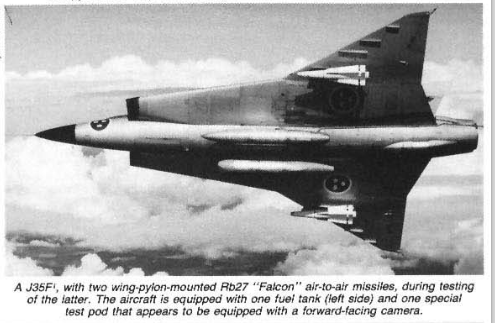
\includegraphics[width=\textwidth]{S35F}
\end{figure}

\LARGE 
Nikolaos Koukis

\vfill
\normalsize \normalfont
Personnummer: 930727T073\\
Date delivered: 2015/02/03\\
Group: D
\end{center}
\end{titlepage}

\newpage
\tableofcontents
\listoffigures
\lstlistoflistings
\newpage

%%%%%%%%%%%%%%%%%%%%%%%%%%%%%%%%%%%%%%%
%           ABSTRACT                  %
%%%%%%%%%%%%%%%%%%%%%%%%%%%%%%%%%%%%%%%
\section{Abstract}
This is the report for the performance analysis project in the \textit{Flight Mechanics} course
offered by the School of Engineering Sciences at KTH. The report was written using the \textit{Vim} Editor
and the \XeLaTeX typesetting system. For the coding part the \textit{Matlab} technical computing language was used.



%%%%%%%%%%%%%%%%%%%%%%%%%%%%%%%%%%%%%%%
%           ABSTRACT                  %
%%%%%%%%%%%%%%%%%%%%%%%%%%%%%%%%%%%%%%%
\section{Introduction}

\subsection{General Characteristics}
As the jet era started, Sweden foresaw the need for a jet fighter that could intercept bombers at high 
altitude and also successfully engage fighters. Although other interceptors such as the 
US Air Force's F-104 Starfighter were being conceived during the same period, 
Saab's "Draken" would have to undertake a combat role unique to Sweden. 
Other demanding requirements were the capability to operate from reinforced public roads 
used as part of wartime airbases, and for refuelling/rearming to be 
carried out in no more than ten minutes, by conscripts with minimal training. 
\textbf{In September 1949, the Swedish Defence Material Administration issued a request for a fighter/interceptor aircraft, and work began at Saab the same year}

\textit{Regarding the aerodynamic design of the J35 Draken the two major options were swept wings and delta wings.}
The question was quickly resolved by the initial studies which had called for the
exploration of a swept wing configuration. In short order it  was determined tha
in consideration of all other parameteres placed upon the design, 
the swept wing's aerodynamic drag at high Mach numbers was too high, 
and its configuration requirements dictated that the fuselage have insufficient 
volume for equipment, fuel and armament.
The Delta wing on the other hand showed great promise following initial tunnel 
tests. The pure delta soon was ruled out, however, as it suffered from center 
of gravity and center of pressure anomalies that were difficult to alleviate. 
A derivative, however, often referred to as \textit{the double delta}, proved much more flexible. 
In general the double delta was found to offer the attributes of:
\begin{itemize*}
    \item reduced frontal area while permitting optimal wing area
    \item More favorable wing sweep angles on the center wing section
    \item Center of gravity and center of pressure being closer to each other
    \item More favorable area distribution
    \item Low supersonic drag
    \item Favorable low speed drag
    \item Strong and stiff fail safe structure
    \item Being able to place the air intakese farther forward
\end{itemize*}
The double-delta configuration was first tested on the SAAB 210 which first flew
on 21 January 1952.

\begin{figure}[H]
  \centering
  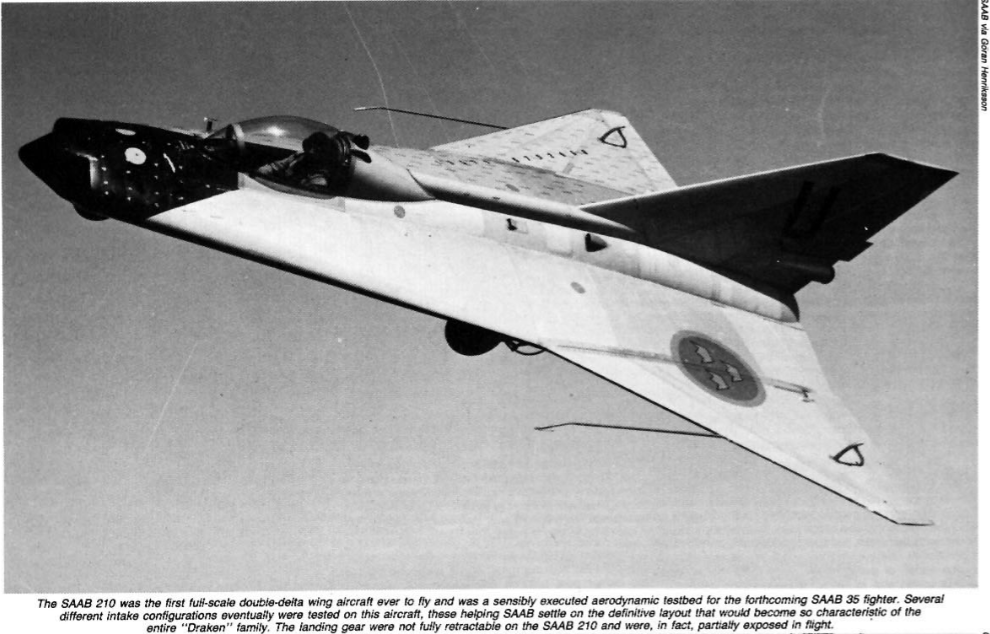
\includegraphics[width=1.2\textwidth]{SAAB210}
  \caption{SAAB 210}
\end{figure}
\begin{figure}[H]
  \centering
  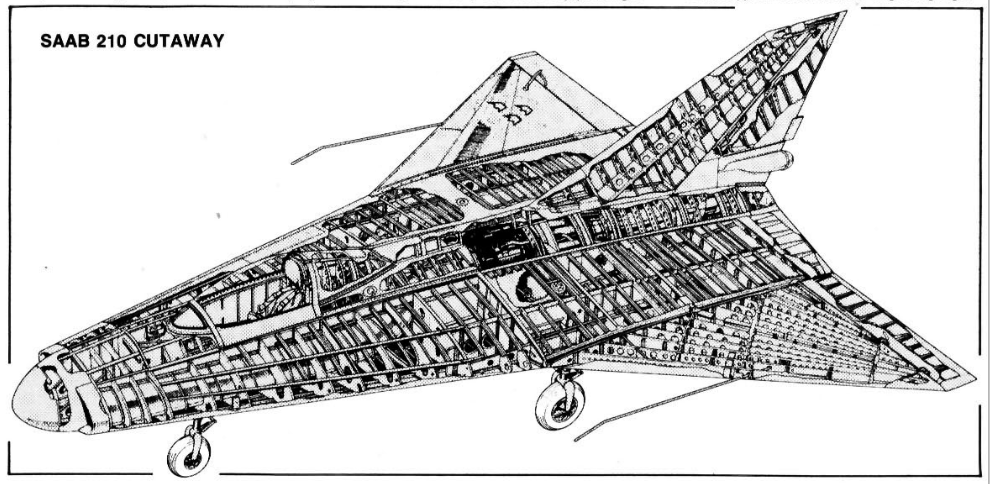
\includegraphics[width=1.3\textwidth]{Cutaway}
  \caption{Cutaway design of SAAB 210}
\end{figure}

\subsection{Basic Versions}

Below are the major versions of J35 Draken which were manufactured from 1955
to 1974 by Saab.
\subsubsection{J35A}

    \begin{itemize*}
        \item First flew on 1958
        \item Total Production: 90
        \item Delivered from 1959 to 1961
    \end{itemize*}

\begin{figure}[H]
  \centering
  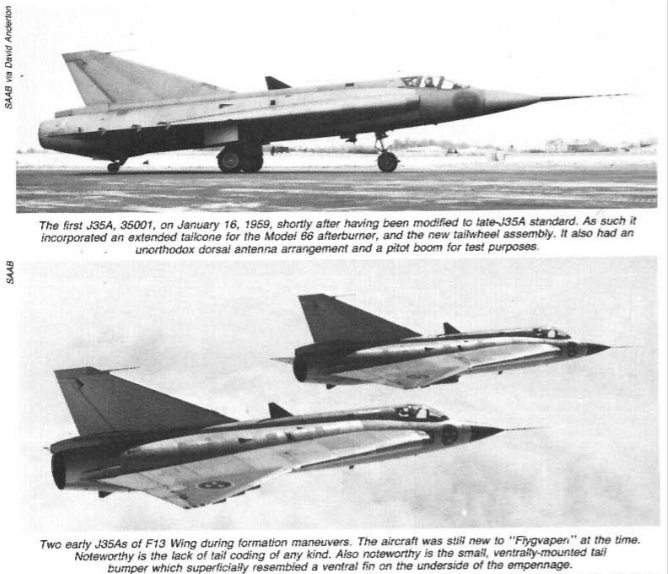
\includegraphics[width=1.0\textwidth]{J35A}
  \caption{J35A}
\end{figure}
\subsubsection{J35B}
\begin{itemize*}
        \item First flew on 1959
        \item Total Production: 73
        \item Delivered from 1962 to 1963
        \item First truly operating interceptor version of J35 Draken
    \end{itemize*}

\begin{figure}[H]
    \centering
    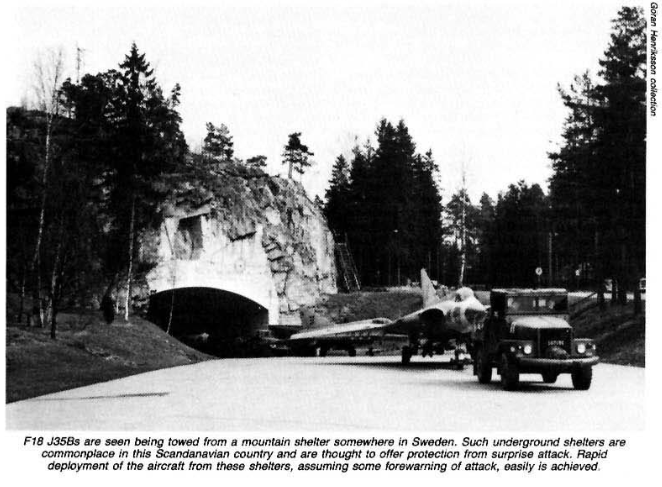
\includegraphics[width=1.0\textwidth]{S35b_sheltered}
    \caption{J35B carried out of sheltered area}
\end{figure}

\begin{figure}[H]
    \centering
    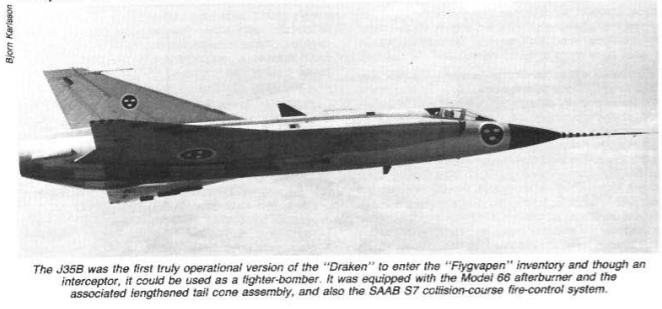
\includegraphics[width=1.0\textwidth]{S35B}
    \caption{J35B}
\end{figure}

\subsubsection{Sk35C}
    \begin{itemize*}
        \item First flew on 1959
        \item Total Production: -
        \item Essentially 25 J35A with short tail sections rebuilt 
            into a twin-seated trainer version
        \item To provide space for a second cockpit some equipment was relocated and the size of the forward
            fuel tank was reduced.
        \item Lacking the guns and radar of single-seater, the Sk35C nevertheless could be 
            used for armament training with Sidewinder missiles and other external stores.
    \end{itemize*}

\begin{figure}[H]
  \centering
  \hspace*{-2cm} 
  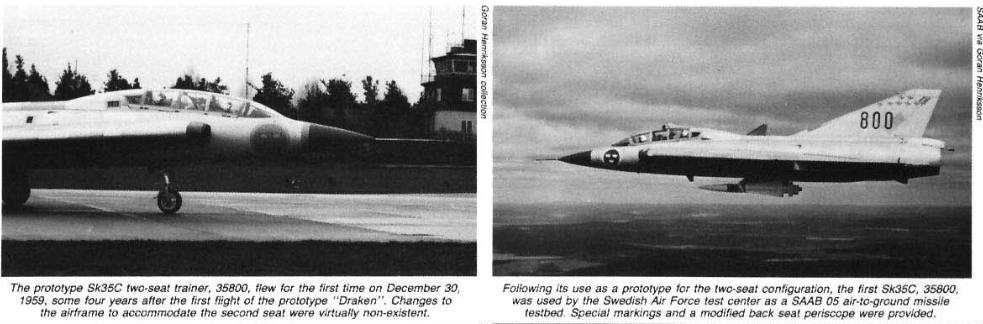
\includegraphics[width=1.2\textwidth]{Sk35C}
  \caption{Sk35C}
\end{figure}

\subsubsection{J35D}
    \begin{itemize*}
        \item First flew on 1960
        \item Total Production: 120
        \item Delivered from 1963 to 1964
        \item Fastest Draken version, capable of accelerating until out of fuel.
        \item Represented a marked improvement over earlier versions both in terms of performance and combat capabillities.
            The former was obtained by replacing the RM5B engine with RM5C (Avon-300 series) thus increasing the max thrust forom 6.850 kgp to 7.750 kgp
            when using the afterburner.
    \end{itemize*}

\begin{figure}[H]
  \centering
  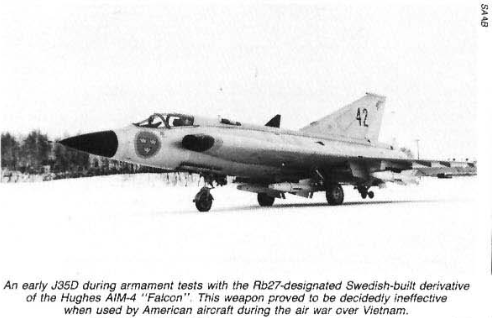
\includegraphics[width=1.0\textwidth]{J35D}
  \caption{J35D}
\end{figure}

\subsubsection{S35E}
    \begin{itemize*}
        \item Total Production: 60
    \end{itemize*}


\begin{figure}[H]
    \centering
    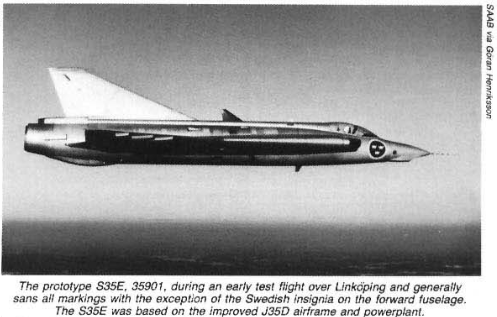
\includegraphics[width=\textwidth]{S35E}
    \caption{J35E}
\end{figure}
\begin{figure}[H]
    \centering
    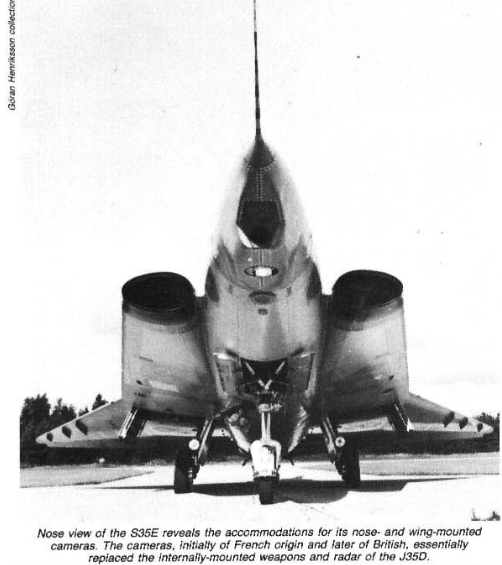
\includegraphics[width=\textwidth]{S35E_b}
    \caption{J35E nose view}
\end{figure}

\subsubsection{S35F}
\begin{figure}[H]
    \centering
    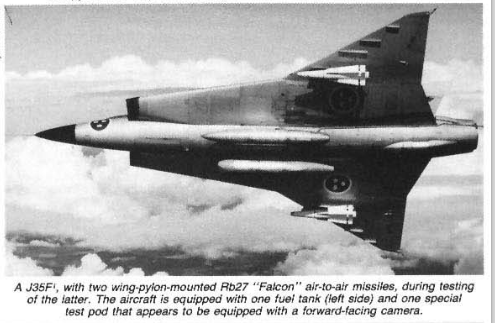
\includegraphics[width=\textwidth]{S35F}
    \caption{J35F}
\end{figure}
\begin{figure}[H]
    \centering
    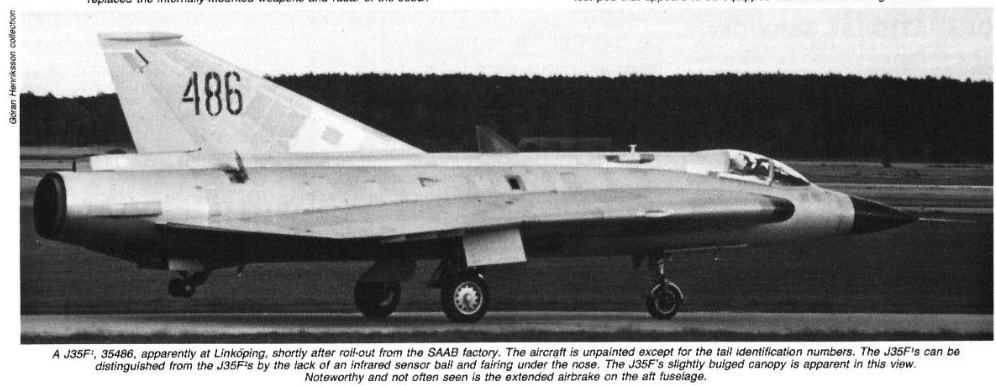
\includegraphics[width=\textwidth]{S35F_b}
    \caption{J35F landing}
\end{figure}

\subsubsection{S35H}
Version of J35 which was supposed to be sold to Switzerland by SAAB. During 1960 it 
was evaluated thoroughly in Switzerland with generally favorable results.
The J35H was not however the only aircraft considered and in the end the Schweizerische
Fliegertruppe concluded that a slightly modified version of Dassault Mirage III was more ideally suited.

\subsubsection{SAAB 35XD}
\begin{itemize*}
    \item Company designation in which X stoood for export and D for Denmark
    \item In 1968 The Danish Goverment ordered 20 single seated 3 two seated trainers 
        23 photo-reconnaissance aircrafts in a follow up order. Finally the Danes revised their offer for 20 single seat 
        20 reconnaisance aircrafts and 11 two-seat trainers.
\end{itemize*}

\subsubsection{SAAB 35XS}
\begin{itemize*}
    \item Export version for Suomi or Finland
    \item Ordered during 1970 by Finland
\end{itemize*}


%%%%%%%%%%%%%%%%%%%%%%%%%%%%%%%%%%%%%%%
%        STATIC ANALYSIS              %
%%%%%%%%%%%%%%%%%%%%%%%%%%%%%%%%%%%%%%%
\subsection{Static Perfomance}

\subsection{Excess Thrust}

Figure \ref{fig:Tex_Graph} shows the Excess Thrust with regards to the Mach number is presented:

\begin{figure}[H]
    \centering
    \hspace*{-2cm}
    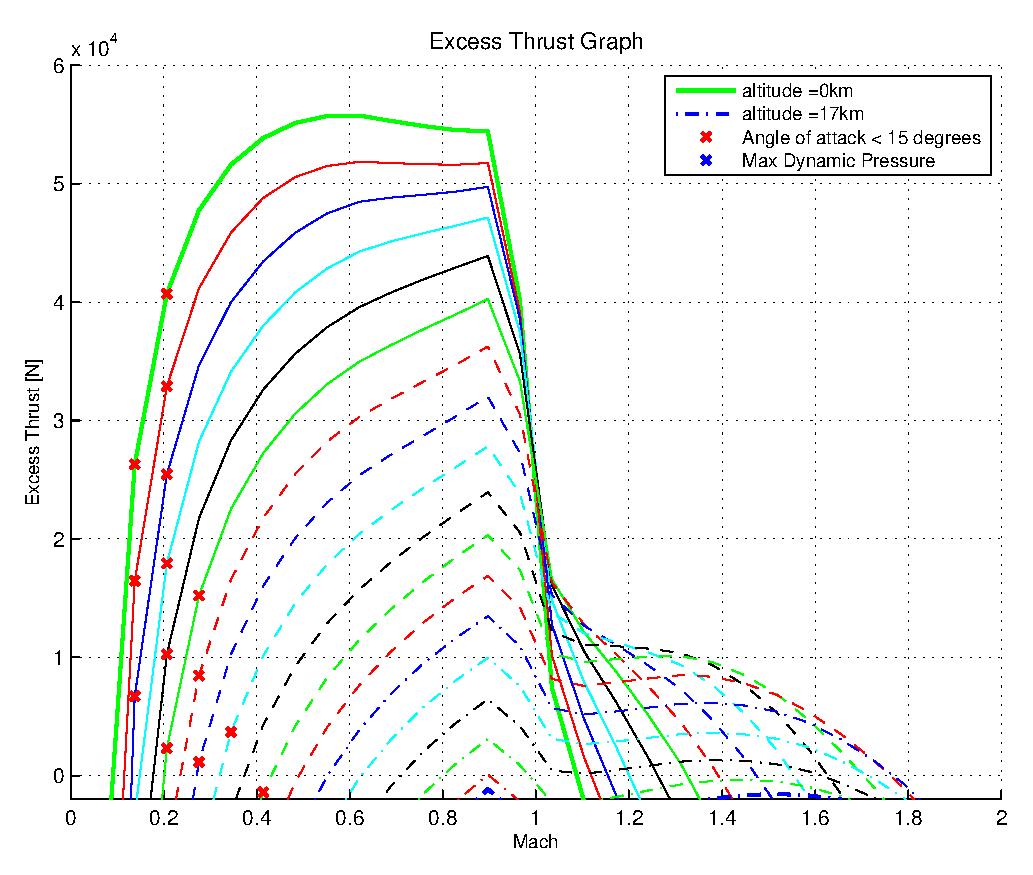
\includegraphics[width=1.2\textwidth]{Tex_Graph}
    \caption{Excess Thrust Graph}
    \label{fig:Tex_Graph}
\end{figure}

Using the graph we can now determine the envelope limits corresponding to the dynamic pressure and the 
maximum angle of attack. These limits are shown in the diagram as red and blue Xs.
We should note however that the dynamic pressure limits are not visible in  \ref{fig:Tex_Graph}, when presenting 
only the part of the diagram above the zero horizontal line, so a supplementary graph (\ref{fig:Tex_Graph2}) is given:

\begin{figure}[H]
    \centering
    \hspace*{-2cm}
    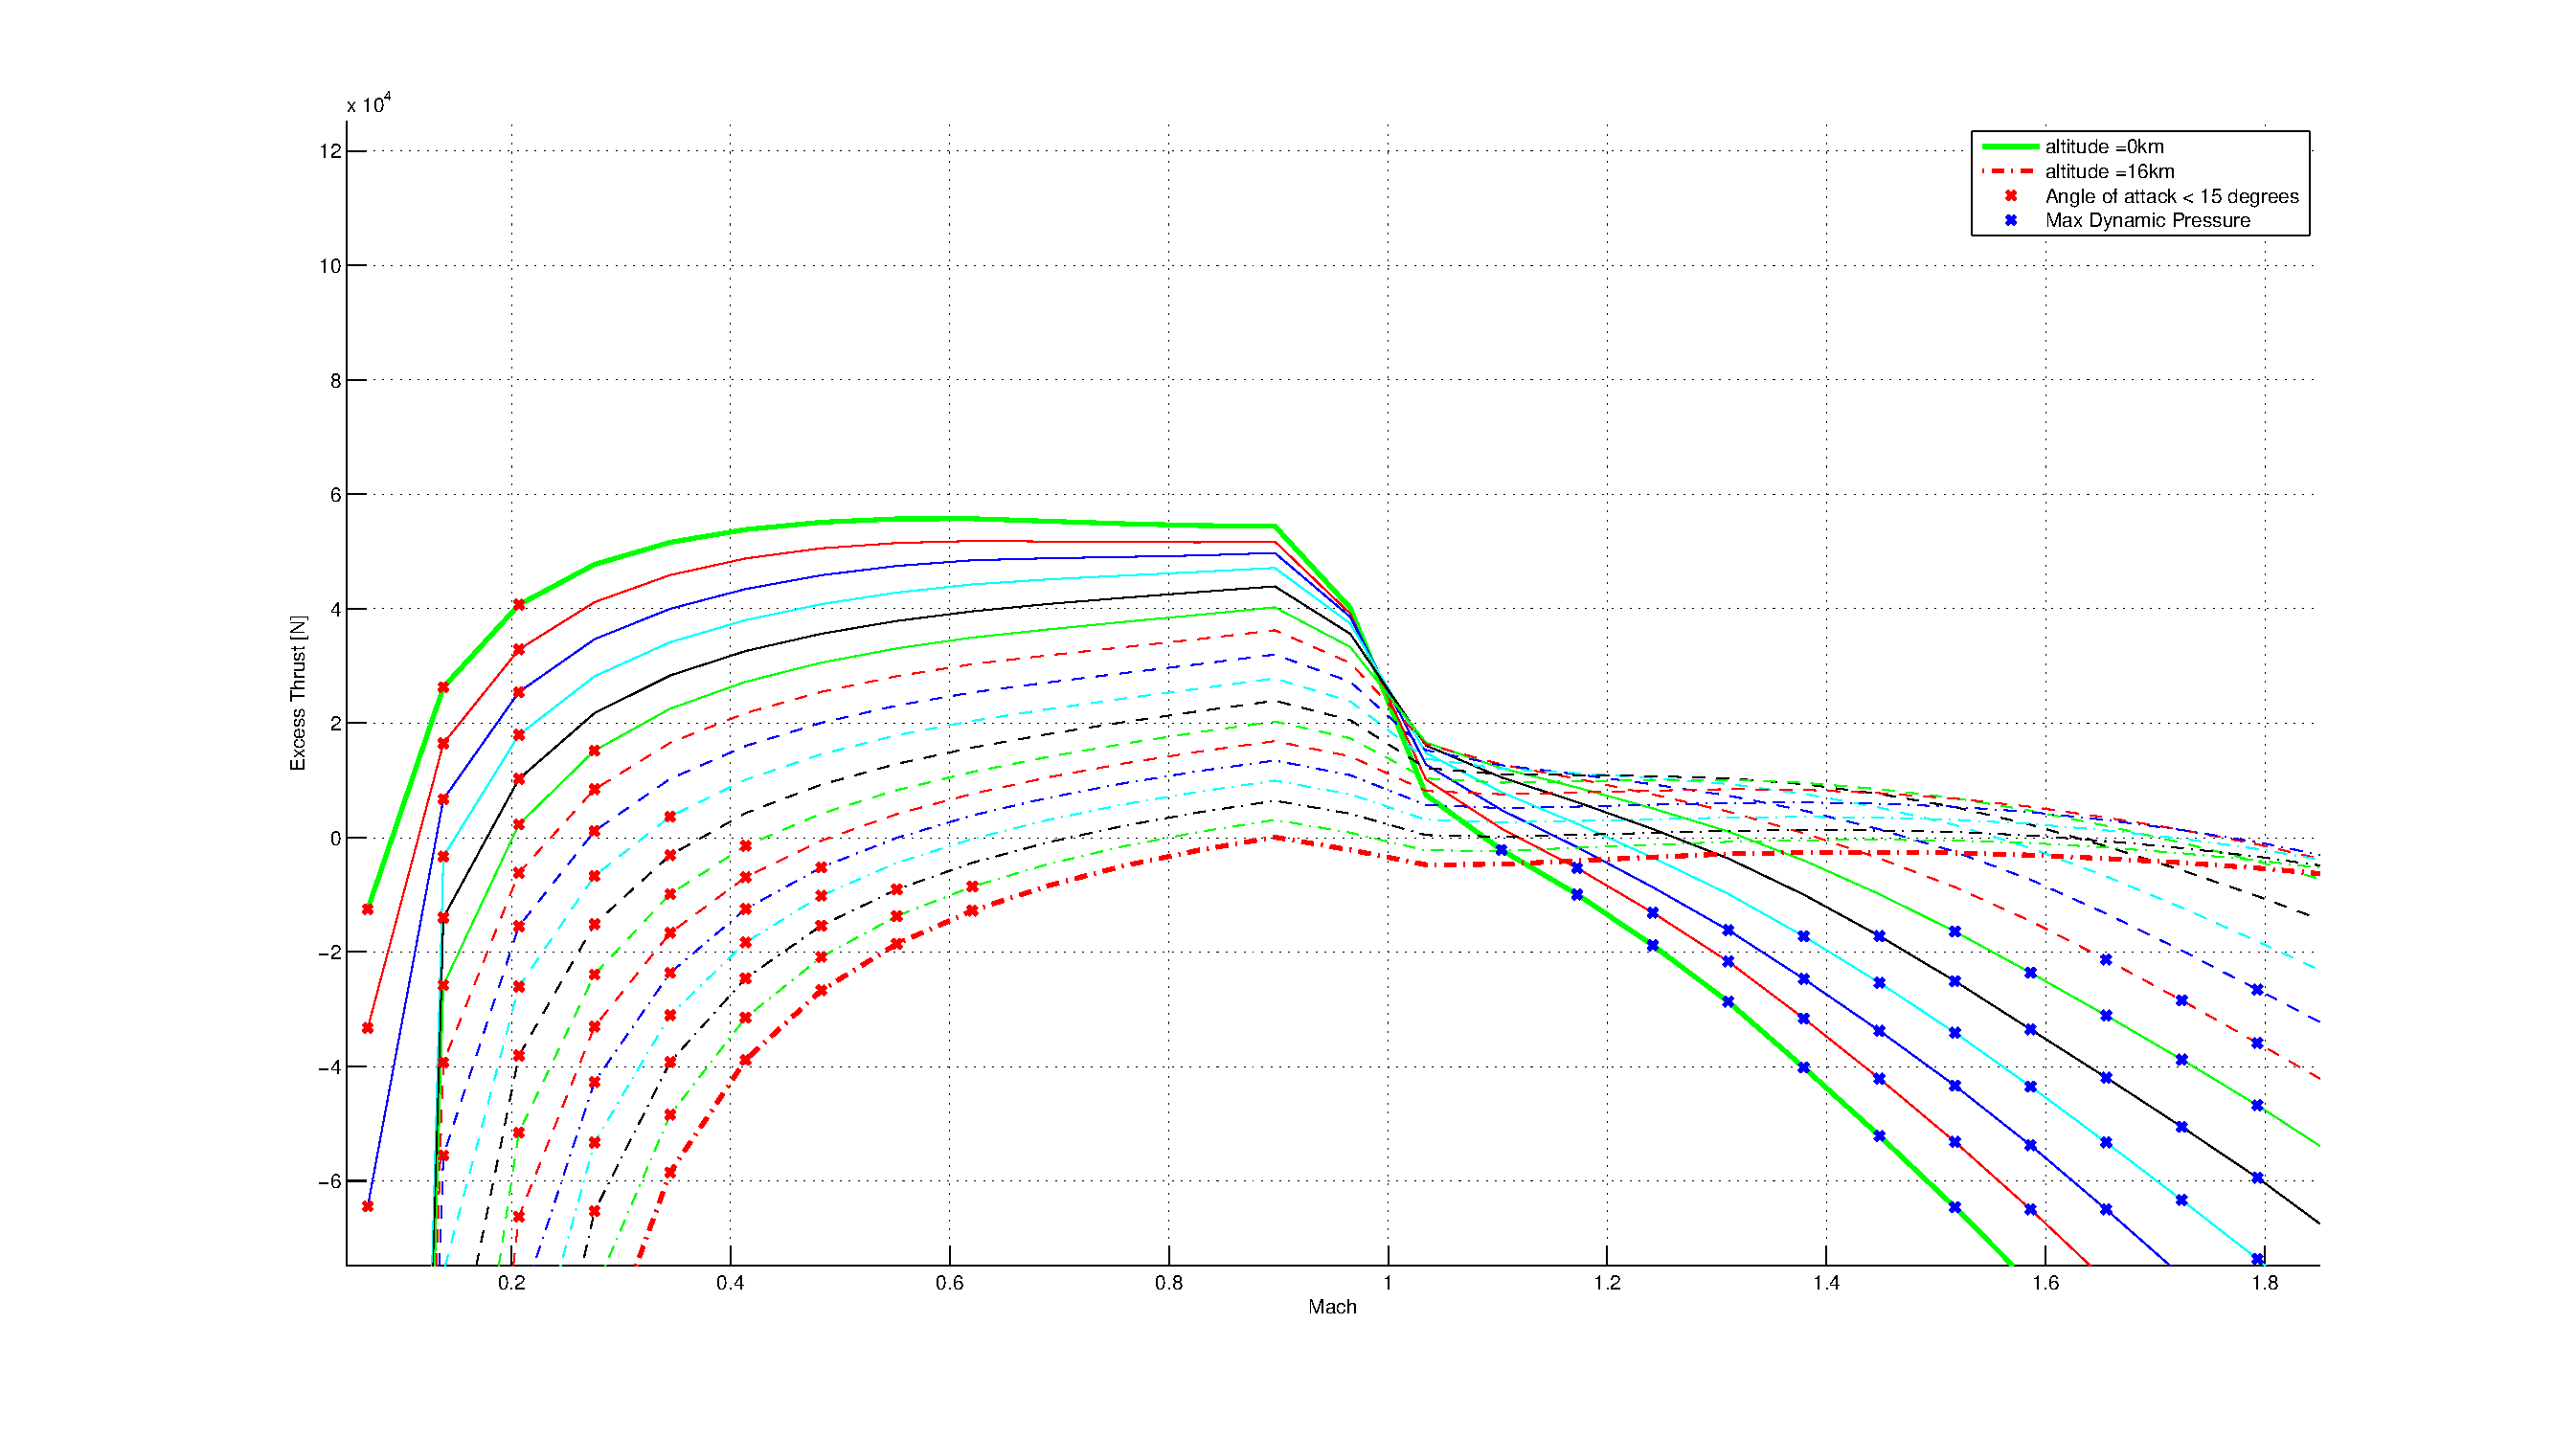
\includegraphics[width=1.2\textwidth]{Tex_Graph2}
    \caption{Excess Thrust Graph - Dynamic pressure limits Visible}
    \label{fig:Tex_Graph2}
\end{figure}

\noindent For the calculation of the Excess Thrust the TexSep function was used. Refer to the TexSep.m module 
for more information on the implementation

\subsection{SEP Graph}

Using the code provided with the report the Specific Excess Power (SEP) Graph
can be plotted:

\begin{figure}[H]
    \centering
    \hspace*{-2cm}
    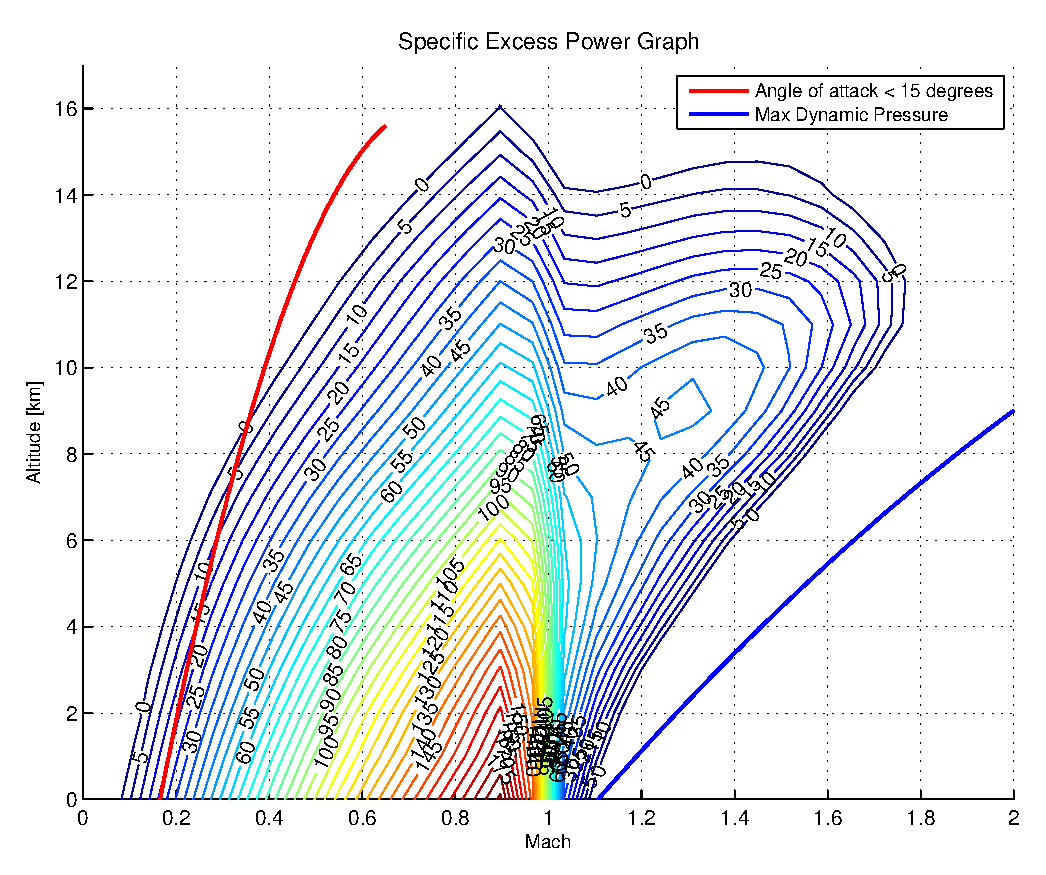
\includegraphics[width=1.2\textwidth]{SEP_Graph}
    \caption{SEP Graph}
    \label{fig:SEP_Graph}
\end{figure}

Graph \ref{fig:SEP_Graph} shows the contours of same Excess Power with regards to
the altitude of the airplane as well as the Mach number thus the velocity of the airplane.

Using the graph we can also determine the envelope limits corresponding to the maximum angle of attack
$(15^{\degree})$ and the maximum dynamic pressure corresponding to $1350 \sfrac{km}{h}$ at sea level which 
is $8.6133e+04 Pa$.

\subsection{Maximum altitude - Maximum Mach Number}
The maximum altitude and the maximum Mach Number at which the aircraft can fly level 
can be determined using \ref{fig:SEP_Graph}:

\begin{itemize*}
    \item Max. Altitude: 16 km
    \item Max Mach: 1.76
\end{itemize*}


%%%%%%%%%%%%%%%%%%%%%%%%%%%%%%%%%%%%%%%
%      MINIMUM TIME TO CLIMB          %
%%%%%%%%%%%%%%%%%%%%%%%%%%%%%%%%%%%%%%%
\section{Minimum time to climb}

\subsection{Computing $\gamma(t)$  - minimum time to climb}

\subsection{Trajectory for maximum Mach number in minimum time}

\subsection{Trajectory for maximum altitude in minimum time}


%----------------------------------------------------------------------------------------
%  BIBLIOGRAPHY
%----------------------------------------------------------------------------------------
\newpage
\nocite{*}
\bibliographystyle{plain}
\bibliography{j35_draken}


\end{document}
